\documentclass[9pt,twocolumn,twoside]{gsajnl}

\articletype{inv} % article type
% {inv} Investigation 
% {gs} Genomic Selection
% {goi} Genetics of Immunity 
% {gos} Genetics of Sex 
% {mp} Multiparental Populations

\title{Microarray-based detection of genomic signatures related with the tumor recurrence in Glioblastoma patients}

\author[$\ast$,1]{Álvaro Abella-Bascarán}
\author[$\ast$]{Eloi Casals-Puig}
\author[$\ast$]{Samuel Miravet-Verde}

\affil[$\ast$]{Pompeu Fabra University, Barcelona (Spain)}

\keywords{Microarray; tumour recurrence; glioblastoma.}

\runningtitle{GENETICS | INVESTIGATION} % For use in the footer 

\correspondingauthor{Corresponding Author}

\begin{abstract}

Glioblastoma tumors, in addition to be the most frequent and aggressive type of brain tumor in humans, are notorious for their resistance to therapy. The aim of this work was to identify which molecular profiles are related with resistance to treatment, by means of the analysis of microarray data from 80 tumor samples (proceeding from the work of \citep{Murat2008}). The analysis led to 
% TODO one line for results in the abstract
\end{abstract}

\setboolean{displaycopyright}{true}

\begin{document}

\maketitle
\thispagestyle{firststyle}
\marginmark
\firstpagefootnote
\correspondingauthoraffiliation{Affiliation correspondence email:  alvaro.abella01@estudiant.upf.edu}

\vspace{-1cm}
\section*{Introduction}

Glioblastoma multiforme is the most frequent and aggressive brain tumor in humans, involving glial cells, with an incidence of 2–3 cases per 100,000 person life-years in Europe and North America \citep{Bleeker2012}. Its treatment can involve chemotherapy, radiation and surgery. Median survival with standard-of-care radiation and chemotherapy with the alkylating agent temozolomide is only 15 months  \citep{Johnson2012} while the median survival without treatment is 4 and a half months. 

Regretfully glioblastomas are notorious for resistance to therapy, which has been attributed to DNA-repair proficiency, a multitude of deregulated molecular pathways, and, more recently, to the particular biologic behavior of tumor stem-like cells, as it is exposed in the work of Anastasia Murat \citep{Murat2008}. In that case the HOX and EGFR related pathways were identified as differentially expressed using several cluster procedures. However, a deeper analysis based on more general techniques can be able to determine the molecular profiles specific for treatment resistance. To achieve that goal, the same set of gene expression profiles of 80 patients has been used. 

\section*{Materials and Methods}

\subsection*{Tumor Samples and Patient Characteristics}

We analyzed data from 80 frozen glioblastoma samples. The data comprised 70 tumors from initial surgery and 10 samples resected at recurrence. All patients were treated within a phase II or a randomized phase III trial \citep{Stupp2002,Stupp2005}
The study includes 21 females and 55 males, with a a median age of 52 (range, 26 to 70 years). Out of the 76 patients, 28 received radiotherapy treatment only, and 48 received TMZ/radiotherapy treatment.


\subsection*{Gene Expression Profiling}

The microarray data with gene expression profiling was obtained from the Gene Expression Omnibus (GEO) database at http://www.ncbi.nlm.nih.gov/geo/ (accession-number GSE7696). The data had been created from probes prepared with the Enzo BioArray-High Yield Kit (Enzo Life Sciences, Farmingdale, NY) for double amplification and were hybridized to Affymetrix HG-133Plus2.0 GeneChips (Affymetrix, Santa Clara, CA). The data used had been normalized to the expression of the EIF2C3, DNAJA4, and B2M genes that exhibited little variation in the data set \citep{Murat2008}.

\subsection*{Data Analysis and Statistical Methods}
Analyses were carried out in R, a free software environment available at http://www.r-project.org/.

\subsubsection*{Quality assessment:}
the quality of the microarray data was assessed by a variety of quality checks. Raw chip images were visually inspected to ensure the absence of  artifacts. The intensity distributions of the samples showed a similar poisson distribution, without any artifactual distribution. We used the linear probe level model (PLM) \citep{Bolstad2004, Brettschneider2007} to verify the absence of artifacts in the chip pseudoimages created from the weights and residuals of the sample PLM's. We used Normalized Unscaled Standard Errors (NUSE) \citep{Bolstad2004} to evalute the deviation of the chip probsets. Samples with NUSE median value higher than 1.05 were removed. Using the same models, we also evaluated the Relative Log Expression (RLE) values \citep{Bolstad2004, Brettschneider2007} to determine technical biases on particular chips. No particular deviation of the median or the interquartile range was found on any sample. The expression intensities for all probe sets from Affymetrix CEL-files were estimated using robust multiarray average  with probe-level quantile normalization followed by median polish summarization \citep{Irizarry2003} as implemented in the BioConductor software (http://www.bioconductor.org/). The inspection of MA plots ensured the absence of fluorescent intensity dependent biases \citep{Bolstad2004}. After the quality assurance process, no samples were discarded from the analysis.

\subsubsection*{Analysis of batch effect and confounding variables:}
the samples were checked for batch effect, first using hierarchical clustering after measuring the Spearman correlation among samples, and then verifying the absence of batch effects by multidimensional scaling. The presence of confounding variables was assessed by means of principal component analysis, and different sources of heterogeneity were analyzed by surrogate variable analysis \citep{Leek2007}.

\subsubsection*{Differential Expression}: the list of analyzed probes was reduced using a non-specific filtering \citep{Bourgon2010}, eliminating features with little variation (IQR cutoff = 0.5), consistently low signal across samples, or insufficient annotation. The differential expression analysis of microarray data was done with an empirical Bayes method \citep{Smyth2004} implemented in the Bioconductor package limma. The Benjamini-Hochberg procedure was applied for multiple testing correction (false-discovery rates) \citep{Benjamini1995}. We called DE genes at 10\% FDR.

\subsubsection*{Functional Enrichment}: we analysed the enrichment of gene ontology terms (http://www.geneontology.org) for biological processes (GO BP) using a one-tailed Fisher's exact test \citep{Fisher1922}. The significance of the GO terms is computed conditionally to the significance of its child terms \citep{Alexa2006}. GO terms formed by less than five genes or with less than five DE genes were removed to improve the reliability of the results.

\section*{Results and Discussion}


\section*{Additional guidelines}

\subsection*{Numbers} In the text, write out numbers nine or less except as part of a date, a fraction or decimal, a percentage, or a unit of measurement. Use Arabic numbers for those larger than nine, except as the first word of a sentence; however, try to avoid starting a sentence with such a number.

\subsection*{Units} Use abbreviations of the customary units of measurement only when they are preceded by a number: "3 min" but "several minutes". Write "percent" as one word, except when used with a number: "several percent" but "75\%." To indicate temperature in centigrade, use ° (for example, 37°); include a letter after the degree symbol only when some other scale is intended (for example, 45°K).

\subsection*{Nomenclature and Italicization} Italicize names of organisms even when  when the species is not indicated.  Italicize the first three letters of the names of restriction enzyme cleavage sites, as in HindIII. Write the names of strains in roman except when incorporating specific genotypic designations. Italicize genotype names and symbols, including all components of alleles, but not when the name of a gene is the same as the name of an enzyme. Do not use "+" to indicate wild type. Carefully distinguish between genotype (italicized) and phenotype (not italicized) in both the writing and the symbolism.

\section*{Examples of Article Components}
\label{sec:examples}

The sections below show examples of different header levels, which you can use in the primary sections of the manuscript (Results, Discussion, etc.) to organize your content.

\section*{First level section header}

Use this level to group two or more closely related headings in a long article.

\subsection*{Second level section header}

Second level section text.

\subsubsection*{Third level section header:}

Third level section text. These headings may be numbered, but only when the numbers must be cited in the text. 

\section*{Figures and Tables}

Figures and Tables should be labelled and referenced in the standard way using the \verb|\label{}| and \verb|\ref{}| commands.

\subsection*{Sample Figure}

Figure \ref{fig:spectrum} shows an example figure.

\begin{figure}[htbp]
\centering
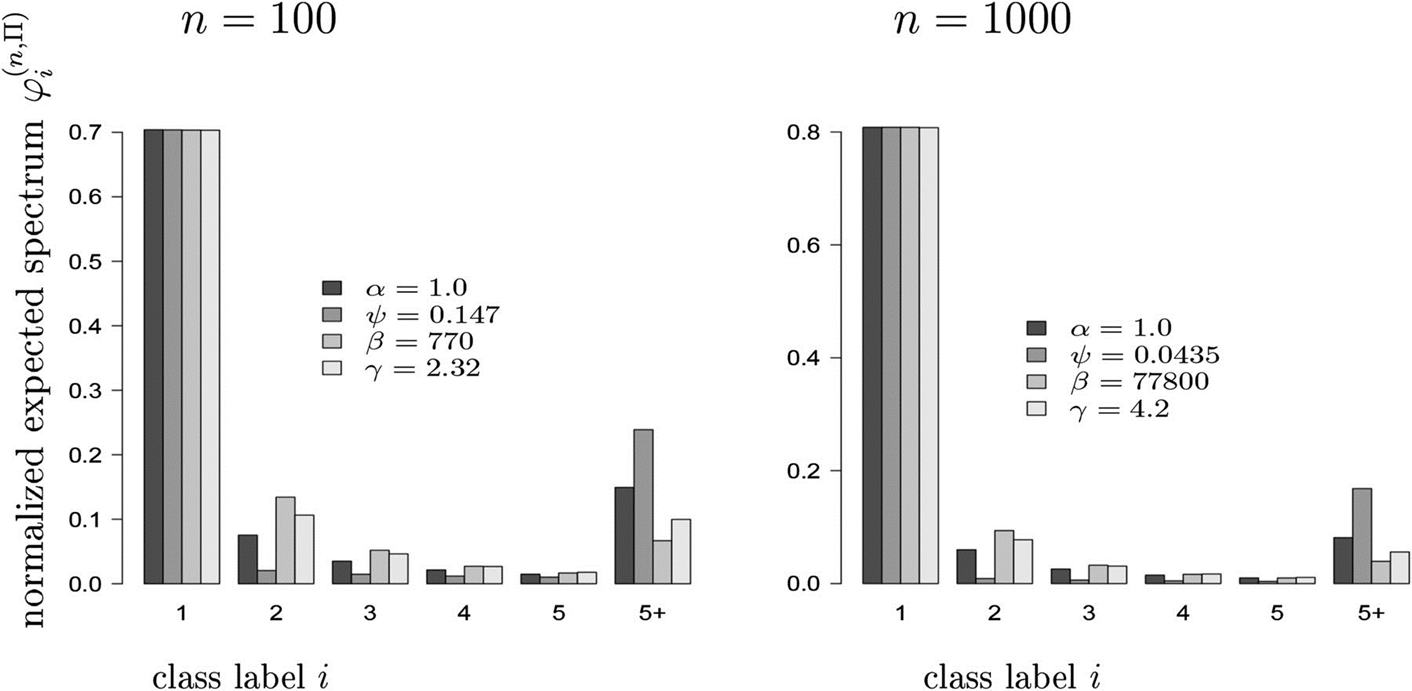
\includegraphics[width=\linewidth]{example-figure}
\caption{Example figure from \url{10.1534/genetics.114.173807}. Please include your figures in the manuscript for the review process. You can upload figures to Overleaf via the Project menu. Upon acceptance, we'll ask for your figure files to be uploaded in any of the following formats: TIFF (.tiff), JPEG (.jpg), Microsoft PowerPoint (.ppt), EPS (.eps), or Adobe Illustrator (.ai).  Images should be a minimum of 300 dpi in resolution and 500 dpi minimum if line art images.  RGB, CMYK, and Grayscale are all acceptable. Halftones should be high contrast with sharp detail, because some loss of detail and contrast is inevitable in the production process. Figures should be 10-20 cm in width and 1-25 cm in height. Graph axes must be exactly perpendicular and all lines of equal density.
Label multiple figure parts with A, B, etc. in bolded type, and use Arrows and numbers to draw attention to areas you want to highlight. Legends should start with a brief title and should be a self-contained description of the content of the figure that provides enough detail to fully understand the data presented. All conventional symbols used to indicate figure data points are available for typesetting; unconventional symbols should not be used. Italicize all mathematical variables (both in the figure legend and figure) , genotypes, and additional symbols that are normally italicized.  
}%
\label{fig:spectrum}
\end{figure}

\subsection*{Sample Video}

Figure \ref{video:spectrum} shows how to include a video in your manuscript.

\begin{figure}[htbp]
\centering
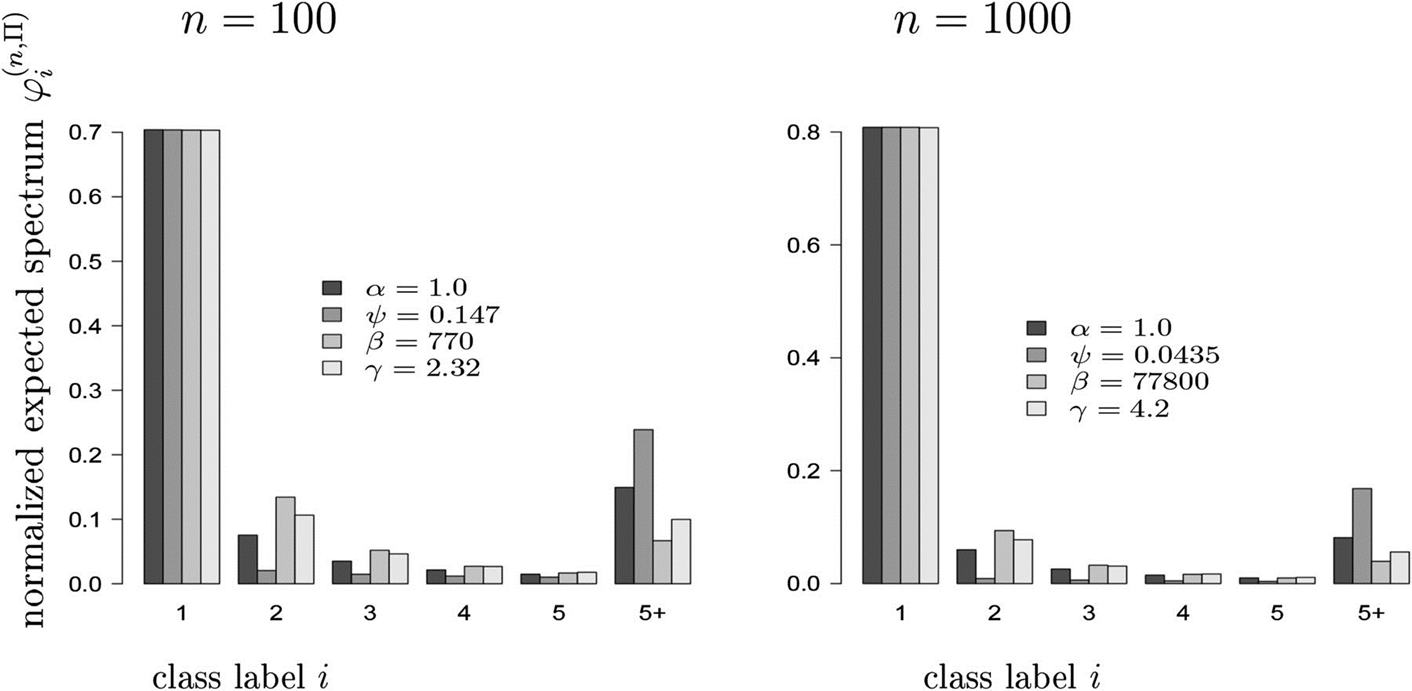
\includegraphics[width=\linewidth]{example-figure}
\caption{Example movie (the figure file above is used as a placeholder for this example). \textit{GENETICS} supports video and movie files that can be linked from any portion of the article - including the abstract. Acceptable formats include .asf, avi, .wav, and all types of Windows Media files.   
}%
\label{video:spectrum}
\end{figure}


\subsection*{Sample Table}

Table \ref{tab:shape-functions} shows an example table. Avoid shading, color type, line drawings, graphics, or other illustrations within tables. Use tables for data only; present drawings, graphics, and illustrations as separate figures. Histograms should not be used to present data that can be captured easily in text or small tables, as they take up much more space.  

Tables numbers are given in Arabic numerals. Tables should not be numbered 1A, 1B, etc., but if necessary, interior parts of the table can be labeled A, B, etc. for easy reference in the text.  


\begin{table*}[htbp]
\centering
\caption{\bf Students and their grades}
\begin{tableminipage}{\textwidth}
\begin{tabularx}{\textwidth}{XXXX}
\hline
Student & Grade\footnote{This is an example of a footnote in a table. Lowercase, superscript italic letters (a, b, c, etc.) are used by default. You can also use *, **, and *** to indicate conventional levels of statistical significance, explained below the table.} & Rank & Notes \\
\hline
Alice & 82\% & 1 & Performed very well.\\
Bob & 65\% & 3 & Not up to his usual standard.\\
Charlie & 73\% & 2 & A good attempt.\\
\hline
\end{tabularx}
  \label{tab:shape-functions}
\end{tableminipage}
\end{table*}

\section*{Sample Equation}

Let $X_1, X_2, \ldots, X_n$ be a sequence of independent and identically distributed random variables with $\text{E}[X_i] = \mu$ and $\text{Var}[X_i] = \sigma^2 < \infty$, and let
\begin{equation}
S_n = \frac{X_1 + X_2 + \cdots + X_n}{n}
      = \frac{1}{n}\sum_{i}^{n} X_i
\label{eq:refname1}
\end{equation}
denote their mean. Then as $n$ approaches infinity, the random variables $\sqrt{n}(S_n - \mu)$ converge in distribution to a normal $\mathcal{N}(0, \sigma^2)$.

\bibliography{example-bibliography}

\end{document}
